\documentclass[conference]{IEEEtran}
\IEEEoverridecommandlockouts

\usepackage{cite}
\usepackage{amsmath,amssymb,amsfonts}

\usepackage{graphicx}
\usepackage{textcomp}
\usepackage{xcolor}
\usepackage{algorithm} 
\usepackage{algpseudocode} 
% Emad Added the bellow packages
\usepackage{todonotes}
\usepackage[inline]{enumitem}
\usepackage{listings}
\usepackage[switch]{lineno}
\lstset{
  numbers=right,
  stepnumber=1,    
  firstnumber=1,
  numberfirstline=true
}

\def\BibTeX{{\rm B\kern-.05em{\sc i\kern-.025em b}\kern-.08em
    T\kern-.1667em\lower.7ex\hbox{E}\kern-.125emX}}
\begin{document}
\linenumbers

\title{Unique Groups on Find Usages}

\author{\IEEEauthorblockN{1\textsuperscript{st} Given Name Surname}
\IEEEauthorblockA{\textit{dept. name of organization (of Aff.)} \\
\textit{name of organization (of Aff.)}\\
City, Country \\
email address}
\and
\IEEEauthorblockN{2\textsuperscript{nd} Given Name Surname}
\IEEEauthorblockA{\textit{dept. name of organization (of Aff.)} \\
\textit{name of organization (of Aff.)}\\
City, Country \\
email address}
\and
\IEEEauthorblockN{3\textsuperscript{rd} Given Name Surname}
\IEEEauthorblockA{\textit{dept. name of organization (of Aff.)} \\
\textit{name of organization (of Aff.)}\\
City, Country \\
email address}

}


% \author{
% \IEEEauthorblockN{Emad Aghayi}
% \IEEEauthorblockA{\textit{Department Of computer Science} \\
% \textit{George Mason University}\\
% Fairfax, VA \\
% eaghayi@gmu.edu}
% \and
% \IEEEauthorblockN{Aaron Massey}
% \IEEEauthorblockA{\textit{Department Of computer Science} \\
% \textit{George Mason University}\\
% Fairfax, VA \\
% amassey5@gmu.edu}
% \and
% \IEEEauthorblockN{Thomas LaToza}
% \IEEEauthorblockA{\textit{Department Of computer Science} \\
% \textit{George Mason University}\\
% Fairfax, VA \\
% tlatoza@gmu.edu}
% % \and
% % \IEEEauthorblockN{3\textsuperscript{rd} Given Name Surname}
% % \IEEEauthorblockA{\textit{Department Of computer Science} \\
% % \textit{George Mason University}\\
% % Fairfax, VA \\
% % email address or ORCID}
% }

\maketitle

\begin{abstract}
Developers face many challenges when trying to understand large codebases. In particular, they have difficulties in understanding the context of how various internal classes, objects, or methods are used in the codebase. We sought to better understand these challenges by conducting a think-aloud user study with 6 participants. The results of the think-aloud experiment highlighted that developers spend considerable time learning to use internal code artifacts. The result also showed developers use the Find Usages/References tool of IDEs to understand code by example. The results of Find Usages can be long tail of results that developers find difficulty mentally parsing. We also found that find usage/reference results' would contain duplicate examples in disparate locations in the user interfaces, adding to the difficulty of parsing. Based on the think-aloud study, we hypothesized that removing duplicate examples and grouping similar examples together would reduce the excise in using the Find Usages/references tool. We designed and implemented a plugin for IntelliJ IDEA that manipulated result of Find Usages and grouped them based on their similarity. After that, we conducted a controlled experiment with 12 more participants to evaluate our approach. Results showed that this aggregation of unique examples is useful.
\end{abstract}

\begin{IEEEkeywords}
Code navigation, information foraging, Find Usages, Find References, large Codebase
\end{IEEEkeywords}


% ***********************************************Introduction***************************************
\section{Introduction}

Developers face many challenges in understanding codebases. Developers are looking for information to understand the codebase. One source for understanding codebase is documentation, but documents are frequently out of date and often poorly written~\cite{documentation}. Another source is reading the codebase. Developers reported understanding existence codebase is one of the most time-consuming activities of software development and reported understanding rationale behind code is serious challenge~\cite{latoza2006maintaining}. Developers spend a significant amount of time navigating and searching existing code for completing their daily tasks~\cite{piorkowski2016foraging,ko2006exploratory}. Developers frequently search for code examples~\cite{brandt2009two,sadowski2015developers}.

Developers prefer to find answer of their questions code rather than documents. Documents are not answering low-level information such as hidden contracts, implementation details, or side effects. Therefore, developers prefer to find the answers in implementation code that could be more accurate and more quick to read~\cite{head2018not}. Developers for finding answers of their questions in the code need tools to navigate and search.\par

Tons of tool exists to help developers to be more productive when they are navigating or searching in codebase~\cite{augustine2015field,ko2006exploratory,albusays2017interviews}. The two most common tools that developers are using in their daily activities are \textit{Find Usages} in Jetbrains IDEs and \textit{Open Call Hierarchy} of Eclipse that Provided this ability for developers. One utilizing example of this tool is that when developers write or edit code, they might come across code elements that they want to change or delete. Before they make changes, they look where the code element is used and how it affects the codebase. Although these tools are the most popular, they have many unaddressed challenges. Results of \textit{Find Usages} are listed in a window in Jetbrains IDEs that developers are going through the results to find the desired usage or understand the codebase. In large codebases, similar usages are frequently happen. Because of that in this kind of codebases, they are facing a high number of duplicate usages.\par

% Another daily issue is navigation from one statement other to task-related code. Sometimes developers want to go through related statements to understand the codebase. Also, they are facing challenges to answer questions about how a change affects callers. When developers want to change an artifact before changing that they check the side effect of that change. They go through the codebase and evaluate the effect of change on them. There exist multiple approaches for better support of structural navigation.\par

% During programming tasks, it is common for a developer to use an object or routine they were previously unfamiliar with. A programmer could also be unfamiliar with how a resource is used within a codebase versus the resource itself. Typically, programmers scour the web for documentation or examples~\cite{brandt2009two,parnin2011measuring}. However, this is not an option for closed source code, forcing developers to rely on internal documentation and examples. Since this may be non-existent or worse (incorrect), example code is a more reliable information source for programmers. The industry-standard approach for finding examples is the Find Usages/References tool. However, when large numbers of references are returned from this tool, it can be not very easy for users to parse the results visually .\par

% Developers, when they write or edit code, they might come across code element that they want to change or delete. Before they make changes, they look where the code element is used and how it affects the codebase. \textit{Find Usages} tool in Jetbrains IDEs and \textit{Open Call Hierarchy} tool of Eclipse Provided this ability for developers. Results of Find Usages are listed in a window in Jetbrains IDEs that developers are going through the results to find the desired usage or understand the codebase. In large codebases similar usages is more possible, because of that in this kind of codebases they are facing with with high number of duplicate usages.\par


To investigate the challenges developers face in using Find Usages, we first conducted an exploratory study. We found that participants sometimes became overwhelmed with the number of results. Instead of investigating more usages, participants instead focused on a single usage as as an example for some time before moving on to investigate other potentially better examples.
Based on these findings, we hypothesized that grouping call sites by similarity may help developers to more rapidly understand how to use a function. \par

To explore this idea, we designed and developed Find Unique Usages, which clusters usages by similarity and displays clusters to the developer. 
To evaluate Find Unique Usages, we conducted  an  experiment where 12 developers implemented a small feature in an open-source codebase. We found that developers with Find Unique Usages were significantly faster, completing their task in 35\% less time.\par

In the rest of this paper, we first review related work. We then describe our exploratory study of the use of find usages. Based on these findings, we then present the design of Find Unique Usages and an evaluation of its use. Finally, we conclude with a discussion of limitations as well as opportunities and future directions.


% ***********************************************Related Work***************************************
\section{Relate Work}
Our work builds on prior studies of code navigation, tools for helping developers navigate and find code examples, and approaches for identifying similar code. 

Developers are using code navigation in their daily activities. For instance, they want to understand what a method does or when it is called or want to understand how to reuse a function by finding examples of code snippets. In fact, they investigate source code. Navigating in source code is described in information foraging theory~\cite{pirolli1999informationforaging}. In software engineering, this theory usually modeled as call graphs. Methods are nodes, and function invocations are edges. Developers have challenges in traversing the call graph in code navigation~\cite{albusays2017interviews}. Navigating and re-finding place of the code that had already been visited is frequent, difficult and distracting~\cite{ko2005eliciting,deline2005towards}.\par 

Tools are trying to help developer to be more productive in the code navigation. These tools are grouped into three categories. The first category is structural relationship traversal. These tools find starting point then traverse relationships to find other related code locations~\cite{karrer2011stacksplorer,augustine2015field,latoza2011visualizing}. Another category is recommender tools. Based on history developers did on similar tasks, they predict relevant elements~\cite{zimmermann2005mining,deline2005easing}. Task context navigation is the last category of code navigation tools. They make it easier to navigate back and forth between task context elements~\cite{ko2006exploratory}. Although there exist several tools for code navigation, code navigation is still challenging for developers~\cite{albusays2017interviews}. 

A common way to edit code is by copying existing code, called code clones~\cite{codeCloneDetection2019}. Sometimes code clone is bad, but there exist many situations that code clone is fine. Developers, because of reasons like basic template, design patterns, or reuse of the definition of specific behavior, use code clones~\cite{kim2004ethnographic,kapser2008cloning}. There exist many tools for detecting bad code clones in codebases~\cite{bellon2007comparison}.\par 

There is much research on information foraging and improving learning by examples~\cite{brandt2009two}. There is also much work in code clones clustering~\cite{codeCloneDetection2019}. As far as these authors are aware, this is the first time work on code clones, and their clustering has been used to help forage for examples within a codebase. Typically code cloning is used to infer duplicate code snippets for refactoring or patching. Researchers have attempted to take relevant pieces from each of these fields, and it is this combination of parts that is the contribution~\cite{kapser2009toward}.\par

Find a similar code in a codebase is one code reuse strategy~\cite{rosson1996reuse}. Developers looking for examples of how to use specific methods or objects~\cite{stylos2006mica,umarji2008archetypal}. Opportunistic developers more likely to use example code rather than systematic developers. There exist techniques for supporting reuse, for instance, IDEs has searching tool that enables developers to search for example across the existing codebase, or IDEs has tool for fining right sequence of methods to complete some tasks that developer already started.\par



% ***********************************************Exploratory Study***************************************
\section{Challenges and Benefits of Using Find Usages tool}
We conducted a think-aloud study to understand better current practice and the challenges developers face using existing approaches. The study was in-person, and their interaction and thoughts were recorded. Researchers vocally recorded the process while asking the participant to think-aloud while conducting the study. The participants were allowed to ask for hints or questions or clarifications, but we must not give answers. We were not looking for successful implementation. We were looking for what developers think about the Find Usages interface, without coaxing the answers we may want out of them.\par
We recruited four participants (P1, P2, P3, P4), two female and two male. The first participant was a graduate computer science student at our institution. The remaining three participants worked as a software developer in the industry, two of them had experienced less than one year, but one of them had more than four years of experience in the industry.\par 
We designed two tasks for the study. The first task was warm-up task it supposed to train participant how to use Find Usages tool. The second task was implementing a logic in a codebase. In the beginning of study, the tasks were piloted with the graduate student participant to make sure the tasks are designed correctly or not. At the and of study, we asked participants to respond to a survey for collecting their experience. In that survey, we asked participants to share with us 1) challenges, if any, they experienced related to finding a method, variable, or anything. 2) challenges, if any, they experienced as they tried to begin work on these tasks. 3) challenges, if any, they experienced related to understanding and working with the provided codebase. 4) challenges, if any, they experienced related to their productivity.

\subsection{Tasks}
\label{tasks}

Participants first completed a warm-up task to familiarize themselves with the Find Usages tool. Participants worked in the Google Guava project, a 772,475 LOC open-source library written in Java. We chose this library because we thought it is a suitable representative of the other java codebases and it is large enough. In order to have participants focus specifically on familiarizing themselves with Find Usages, we asked participants to qualitatively describe the range of integer inputs parameters given to two methods in the codebase. We had participants a maximum of 10 minutes to feel like they had become comfortable with the Find Usages tool.\par

To understand the behavior of developers when they try to change a codebase, we designed second task for developers. The codebase that we chose for this task was FlyingSaucer, a pure Java library for rendering XML, XHTML, and CSS. It contains approximately 99,000 LOC. We removed the statements that create a PDF from the codebase and then asked participants to implement functionality to produce “success.pdf.” We added a constraint on the task. Participants should treat code as closed source code, meaning they cannot find Javadocs online or look for online code examples, but they were free to choose any IDE for accomplishing the task. The study was in person, and it lasts 50 minutes for each participant. 
We collected data from the interaction of developers while they were working on both tasks. 

\subsection{Results of Exploratory Study}

Three of four participants did not know about the Find Usages tool, which was interesting, task 1 helped them to learn Find Usages tool. We gave them information and trained them what is Find Usages tool and how they can use it.\par

Participants completed task two in 49, 20, 42 minutes. One of them used the term "implemented" to mean "usage" frequently. In some cases, participants did not have a strong evidence or reason for understanding the codebase. They were trying to use their feeling. 
\begin{quote}"I do not know how .layout() is used but I am going to use it because it's in this code" - (P2) \end{quote}
\begin{quote}"I feel like this [.layout()] should just work, I hope!" - (P4) \end{quote}

Tasks that we defined looked was similar to what they are doing in their job in the industry. 
\begin{quote}
"Not out of the ordinary [from regular industry/work experience] but still a bit overwhelming"- (P2)
\end{quote}
\begin{quote} "This is just like my job" and "I do this at work all the time, no one knows how anything works but we see how things are used"
- (P3)
\end{quote}
The codebase that we gave participants included unit tests. The interesting thing was that participants were using these unit tests to figure out how methods are invoked and what are the possible input arguments for those methods. They primarily utilized tests as examples. Participants sticks to the specific test case, and usage found, do not go looking for others much until it gets too complex of a usage.

\begin{quote} "Tests are a good example of uses." - (P3)\end{quote}
Two participants had a problem with the size of the codebase.
\begin{quote}"Overwhelmed by the amount of code." - (P2) \end{quote}
\begin{quote}"Large codebases are my biggest fear." - (P4) \end{quote}
The similarity of Find Usages results was a severe issue for the participants since the codebases were reasonably large. The problem is shown in Fig.~\ref{fig:usege}. The IDE was returning many results, which was challenging for participants to extract useful information for undressing the method or object. When doing find usage, much code looked similar, and it was difficult for the participant to parse for participants. Also, this problem was severe when the method they tied to get Find Usages was complex and had complicated call graphs.

\begin{figure}
    \centering
    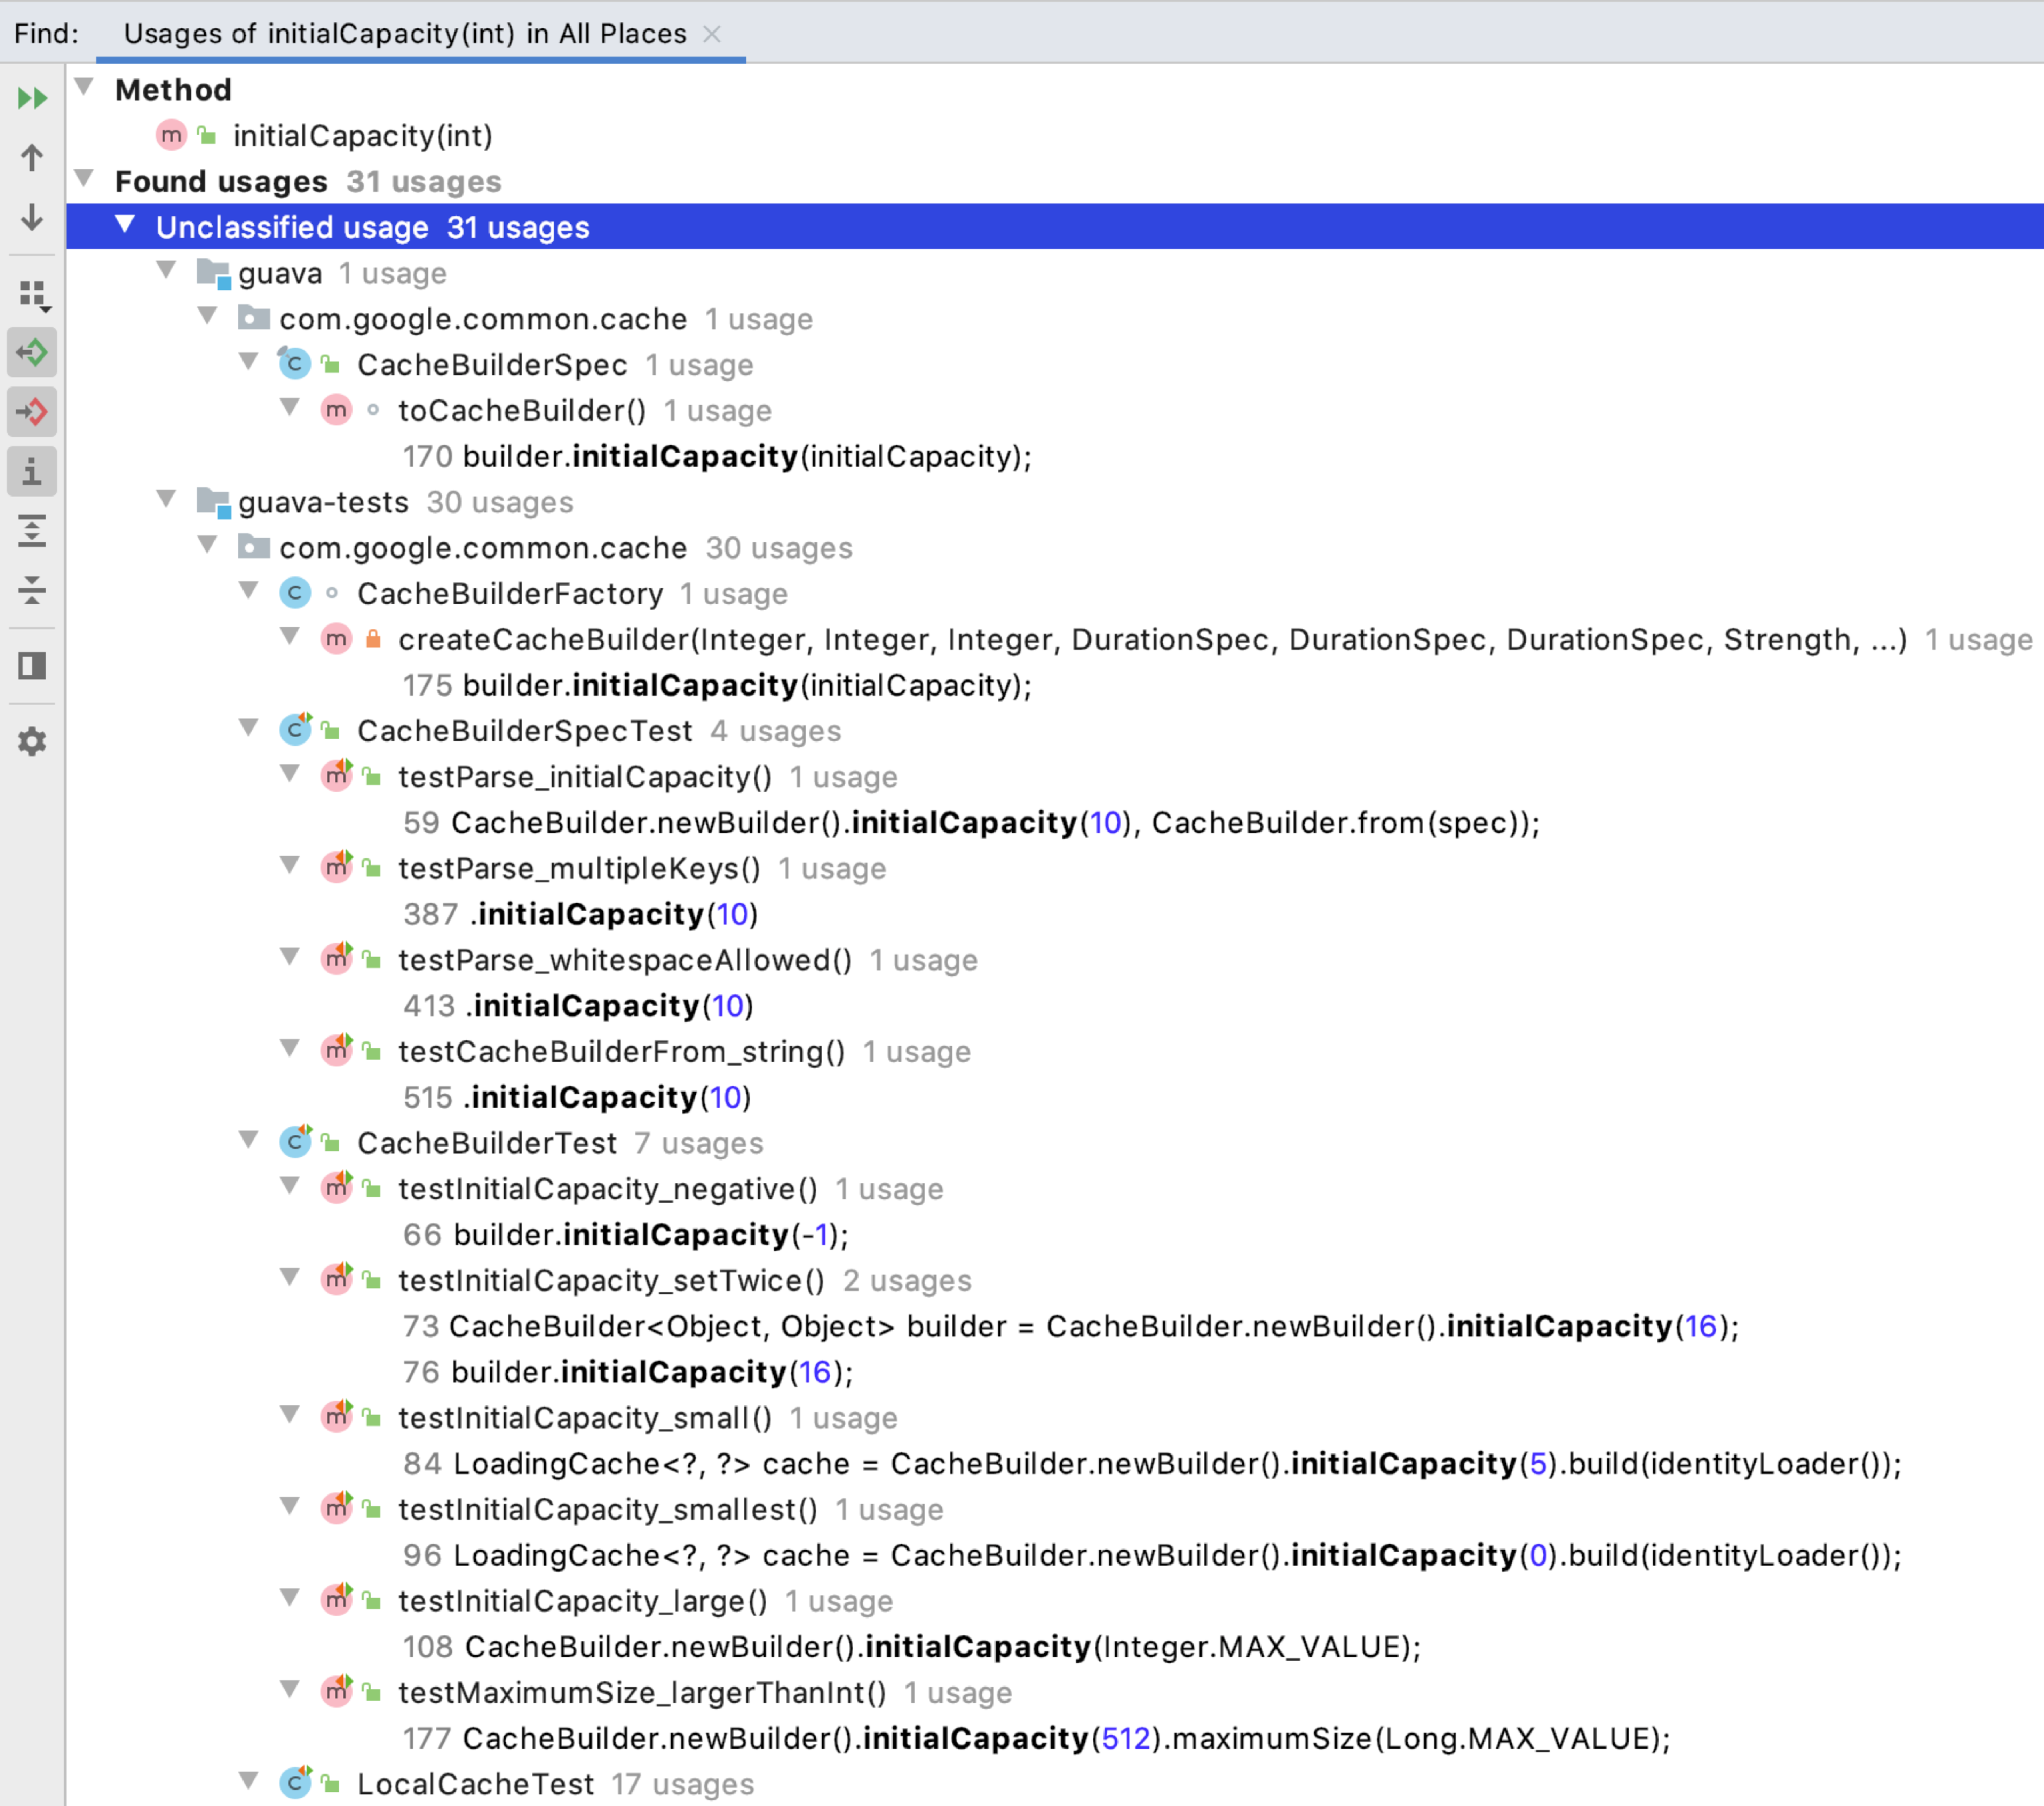
\includegraphics [width=\columnwidth,keepaspectratio, clip]{figures/challenge}
    \caption{It depicts result of regualr Find Usages of IntelliJ IDE. The result window shows there exist 31 usages of the "initCapacity" method. Developers have to go through all of 31 results and also use a pen and paper to find the possible inputs for this method. In this 31 results many of them set same input values of this method, for example 10 is repeated multiple times. This duplicate result is annoying and time consuming for Developers. 
}
\label{fig:usege}
\end{figure}

\begin{quote}"There were a ton of methods and usages that were really similar and it was a lot to put together"- (P4)\end{quote}
\begin{quote}"I had difficulty finding usages with low complexity of calls and uses"- (P4)\end{quote}

Another typical behavior was that participants were scrolling quickly through usages because the surrounding code was not making calls she wanted to make. Participants occasionally navigated to unhelpful usages that took time. A surprising behavior as participants focused on the first result of Find Usage, they copied the first usage, then paste it into the place they want to implement and tried to change it in the way they want.\par 

The confusing thing about Find Usages is happen when a method is overloaded. Participants had difficulty migrating to the correct Find Usages because of overloaded methods.

% ***********************************************System***************************************
\section{Find Unique Usages}
Result of the think-aloud study revealed there exist challenges in using Find Usages tool, participants overwhelmed with tons of usage, and spent substantial time reading through them. We brainstormed on the results and came up with the idea that the refining result of Find Usages might help developers and increase their productivity. In order to design a better tool for addressing the issues, we must understand what is going on in the developers' world and understand how our tool can make the developers' productivity higher. Therefore, we summarized research findings into storyboards. After that, we designed a tool for IntelliJ IDEA that refines the result of the Find Usages tool. The tool aggregates the results and shows the only relevant results. Relevant results likely depend on a measure of sameness.\par
The basic idea behind Find Unique Usages is to group results from a standard Find Usages/References IDE operation based on each result's surrounding code. Our approach is to group usages found by the IntelliJ IDEA usage finder and group them based on similar ASTs while presenting the result to the user. Our comparison leveraged the Gumtree Spoon AST Diff framework, where we measured the resulting differing and matching nodes from an object representing the diff. A general overview of our approach is shown in Fig.~\ref{fig:general} 

\begin{figure*}
    \centering
    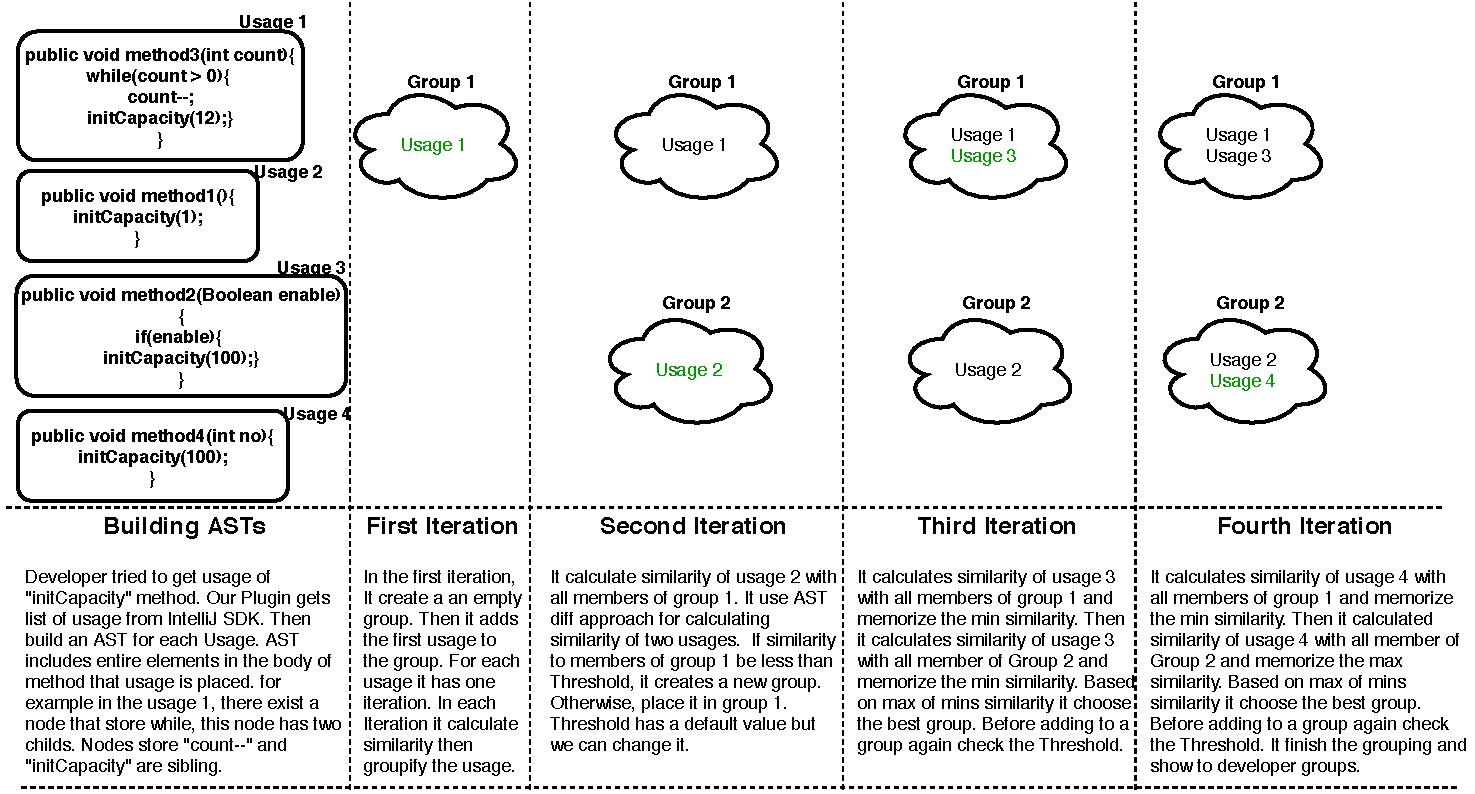
\includegraphics [width=\textwidth,keepaspectratio,clip]{figures/generlView.pdf}
    \caption{This figure depicts how the Find Unique Usages tool works. It collects usages and creates an AST for each usage. Then based on similarity and threshold it decides to assign it to an already exist group or create a new group and assign it to that group. }
\label{fig:general}
\end{figure*}


\subsection{User Interface} 
As adopting unfamiliar tools may impose an additional burden on developers~\cite{adaption2002}, we implemented Find Unique Usages by extending the existing Find Usages interface in the IntelliJ IDE. We added additional usage groups that contained usages with similar code. As each user group contained usages that were surrounded by similar code, we hypothesized the usages would be in similar contexts, implying more information about the usage.Thusa user could inspect one usage within a usage group and gleam that the other usages within that group were similar and move on to another usage group depending on their task. The task we associate this tool with is finding and parsing a large variety of usages while seeking examples of an internal API.

\subsection{Usage Grouping Back-end} 
Usages were grouped based on similar code within the usage's containing method code block. For every usage, IntelliJ IDEA calls our aggregate usage method, which returns a reference to a particular usage group. An internal IntelliJ IDEA object is representing groups of usages. Back-end engine compares the given usage with all other usages in all existing usage groups. The back-end engine consider the given usage to be a part of a usage group when it has a guaranteed minimum threshold of similarity with every abstract syntax tree (AST)  associated with that usage group. If all the usage groups have minimum similarities that do not meet the threshold, then back-end creates a new usage group with the supplied usage and then return that usage group. Logic of the back-end is depicted in Fig.~\ref{fig:flowchart}. \par
\begin{figure}
    \centering
    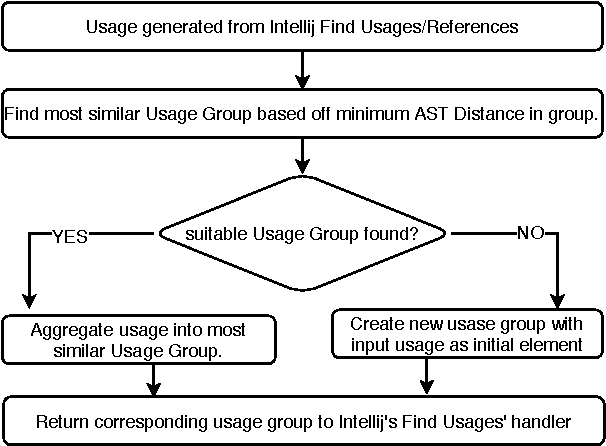
\includegraphics [width=\columnwidth,keepaspectratio, clip]{figures/flowchart}
    \caption{Flowchart shows how the back-end of Find Unique Usages work. }
\label{fig:flowchart}
\end{figure}

The back-end has three main parts. The first part is an algorithm (see Algorithm 1) that it tries to find a minimum similarity between the usage that we want to cluster and all other members of a cluster. It uses the AST diff formula (\ref{equation1}) for calculating the similarity.\par

\begin{algorithm}
\label{algo1}
    \caption{Minimum Similarity in a Usage Group - minSimilarity($x$, $G_{i}$)} 
    \begin{algorithmic}[1]
    \State Given a Usage $x$ and a usage group $G_{i}$
    % \If{$G_{i}$ = null}
    % \State return  $-\infty$
    % \EndIf
    \State $minSimilarity$ $\leftarrow$ $\infty$
    \For{each usage $u_{i}$ in $G_{i}$}
    \State $minSimilarity$$\leftarrow$min($minSimilarity$,similarity($x$,$u_{i}$)) \EndFor
   \State retrun $minSimilarity$
    \end{algorithmic} 
     \
\end{algorithm}

The second main part is an algorithm that tries to find the most similar group for the usage that we want to categorize it, pseudocode of this algorithm is prvided in Algorithm 2. This algorithm iterate over all groups and call Algorithm 1 to find the most similar group. After it finds the most similar cluster to the usage it needs to check another constraint. It needs to consider similarity \textit{threshold}. Finding an appropriate threshold is critical. For example if it choose threshold \textgreater 90\% means very similar, \textgreater 70\% means similar, \textless 40\% means not so similar. A small threshold involves many different usages, and a large threshold might lead to a few results~\cite{deng2013top}. We chose a constant for the similarity threshold of approximately 88\%. There is no real justification for this example besides it working well with an example. We came up with 88\% by doing many trials and errors. In the next step, the algorithm compares the minimum similarity that is calculated with the threshold and based on decide to create a new group or add the usage to the most similar group. 

\begin{algorithm}
\label{algo2}
    \caption{Find Corresponding Usage Group} 
    \begin{algorithmic}[1]
    \State // Given a Usage $x$ \& a set of Usage Groups $G$
    \State $mostSimilarGroup$ $\leftarrow$ $null$
    \For{each Usage Group $G_{i}$ in $G$}
    \If{minSimilarity($x$,$mostSimilarGroup$)$<$ minSimilarity($x$, $G_{i}$)}
    \State $mostSimilarGroup$ $\leftarrow$ $G_{i}$
    \EndIf
    \EndFor
    \State // Given some similarity threshold $T$
    \If{minSimilarity($x$, $mostSimilarGroup$) $<$ $T$}
        \State // Create new usage group and modify $G$.
        \State $G_{new}$ $\leftarrow$ newUsageGroupWithInitialMember($x$)
        \State $G$ $\leftarrow$ $G$ $\cup$ \{$G_{new}$\}
        % \State return $G_{new}$
    \Else
    \State addToGroup($mostSimilarGroup$, $x$)
    % \State return $mostSimilarGroup$
    \EndIf
    \end{algorithmic} 
\end{algorithm}


The last and most important part of our tool is AST diffing approach. Each element in the code can be placed in an AST. The basic problem in similarity of usages was finding a degree of similarity between two usages. The easiest approach is string distance algorithms such as Hamming distance and Levenshtein distance. . Another simplification is decreasing the usage to the lowest level, which is leaf of AST. In our first iteration of creating the tool, we used string distance and considered only the leaf node of the AST that contains the usage. After piloting, we found this naive approach is not fine.\par

Therefore, we made two major changes in the first approach. The first change was that we increased the scope of usage to the entire body of the method that usage placed. In fact, we tried to find similarity among sub-trees instead of leaf nodes of ASTs. Therefore, we increased the scope and consider the entire body of the method that usage places in as a sub-tree. For instance, in the bellow example, if a developer get Find Unique Usage of "add" method, our approach create an AST for usage in line 2. The AST root is name would be "add" it has two children, line 2 and line 3 each be considered as one child node in the AST. Our approach creates  an AST from all elements there exist in the body of method. \par

\begin{lstlisting}[language=Java, caption=AST exmple is shown. Each AST created based on all elements in the body of method.]

    public void callSum(){
        int theSum = add(1, 3);
        System.out.print(theSum);
    }

    public int add(int value1,int value2){
        return value1 + value2;
    }
\end{lstlisting}

Rather than comparing sub-trees for exact match, our approach compares sub-trees similarity based on multiple parameters~\cite{baxter1998clone}. The similarity used a threshold that specifies how similar to sub-trees should be. The formula that computes similarity is:
\begin{equation}
Similarity = 2 \times S  \div (2  \times S  + AST1 + AST2)
\label{equation1}
\end{equation}

where $S$ is number of shared nodes between two trees, $AST1$ is number of different node in AST that hold usage 1, and $AST2$ is number of different node in AST that hold usage 2. \par
Another modification was changing string distance algorithms to a more powerful algorithm. We used GumTree~\cite{baxter1998clone,DBLP:conf/kbse/FalleriMBMM14,falleri2014fine}, which leverage the GumTreeDiff algorithm. We chose this algorithm because GumTreeDiff is focused on fine-grained differentiation that is more sensitive to a programmer~\cite{falleri2014fine}. The Gumtree Spoon AST Diff leverages this algorithm while providing more detailed parsing of Java source code. The authors of GumTreeDiff focus on its use in SCM, where we leverage it for grouping potential example code. \par



% \begin{algorithm}
%     \caption{Similarity of two Usages - similarity($x$, $y$)} 
%     \begin{algorithmic}[1]
%     \State $xAST$  $\leftarrow$ astOfContainingFunction($x$)
%     \State $yAST$ $\leftarrow$ astOfContainingFunction($y$)
%     \State // Get matching AST Nodes in common using gumtree-spoon-ast-diff
%     \State $mappings$ $\leftarrow$ getMappingSet($xAST$, $yAST$)
%     \State 
%     \textbackslash \textbackslash  Use formula from     
%     \State 
%     \textbackslash \textbackslash http://leodemoura.github.io/files/ICSM98.pdf
%     \State $similarity$ $\leftarrow$
%     $$\frac
%     {2*size(mappings)}
%     {2*size(mappings) + size(xAST) + size(yAST)}$$
%     \State return $similarity$
%     \end{algorithmic} 
% \end{algorithm}








% *************************Evaluation section********************************************************************
\section{Evaluation}
To evaluated the tool that we built in terms of productivity, we conducted an experimental user study in which participants tried to add a feature on a codebase. We recruited 12 participants to implement a method and then analyzed their environment interactions and the resulting code they created. 

\subsection{Method}

We recruited 12 more unpaid participants by advertising on our groups of social networks. We use a label for referencing participants. C1, C2,..., C5, C6 worked in control condition. E1, E2,..., E5, E6 worked in the experimental group. 33\% of participants were female, and 66\% were male. Five participants were graduate students, four were working as software developers, and 3 were undergraduates. We randomly assigned participants into a control and experimental condition. All participants used the IntelliJ IDE. Control participants used the Find Usages tool, while experimental participants instead of working with default Find Usage told of IntelliJ IDEA they must work with Find Unique Usages tool. 
Participants again completed the same task as in the exploratory study, described in Section \ref{tasks}. Participants had comparable levels of Java experience, with 60 months for control participants and 62 for experimental participants.\par 
At the end of the study, we conducted a semi-structured interview and asked participants about their experience using the tool.

\begin{figure*}[h]
    \centering
    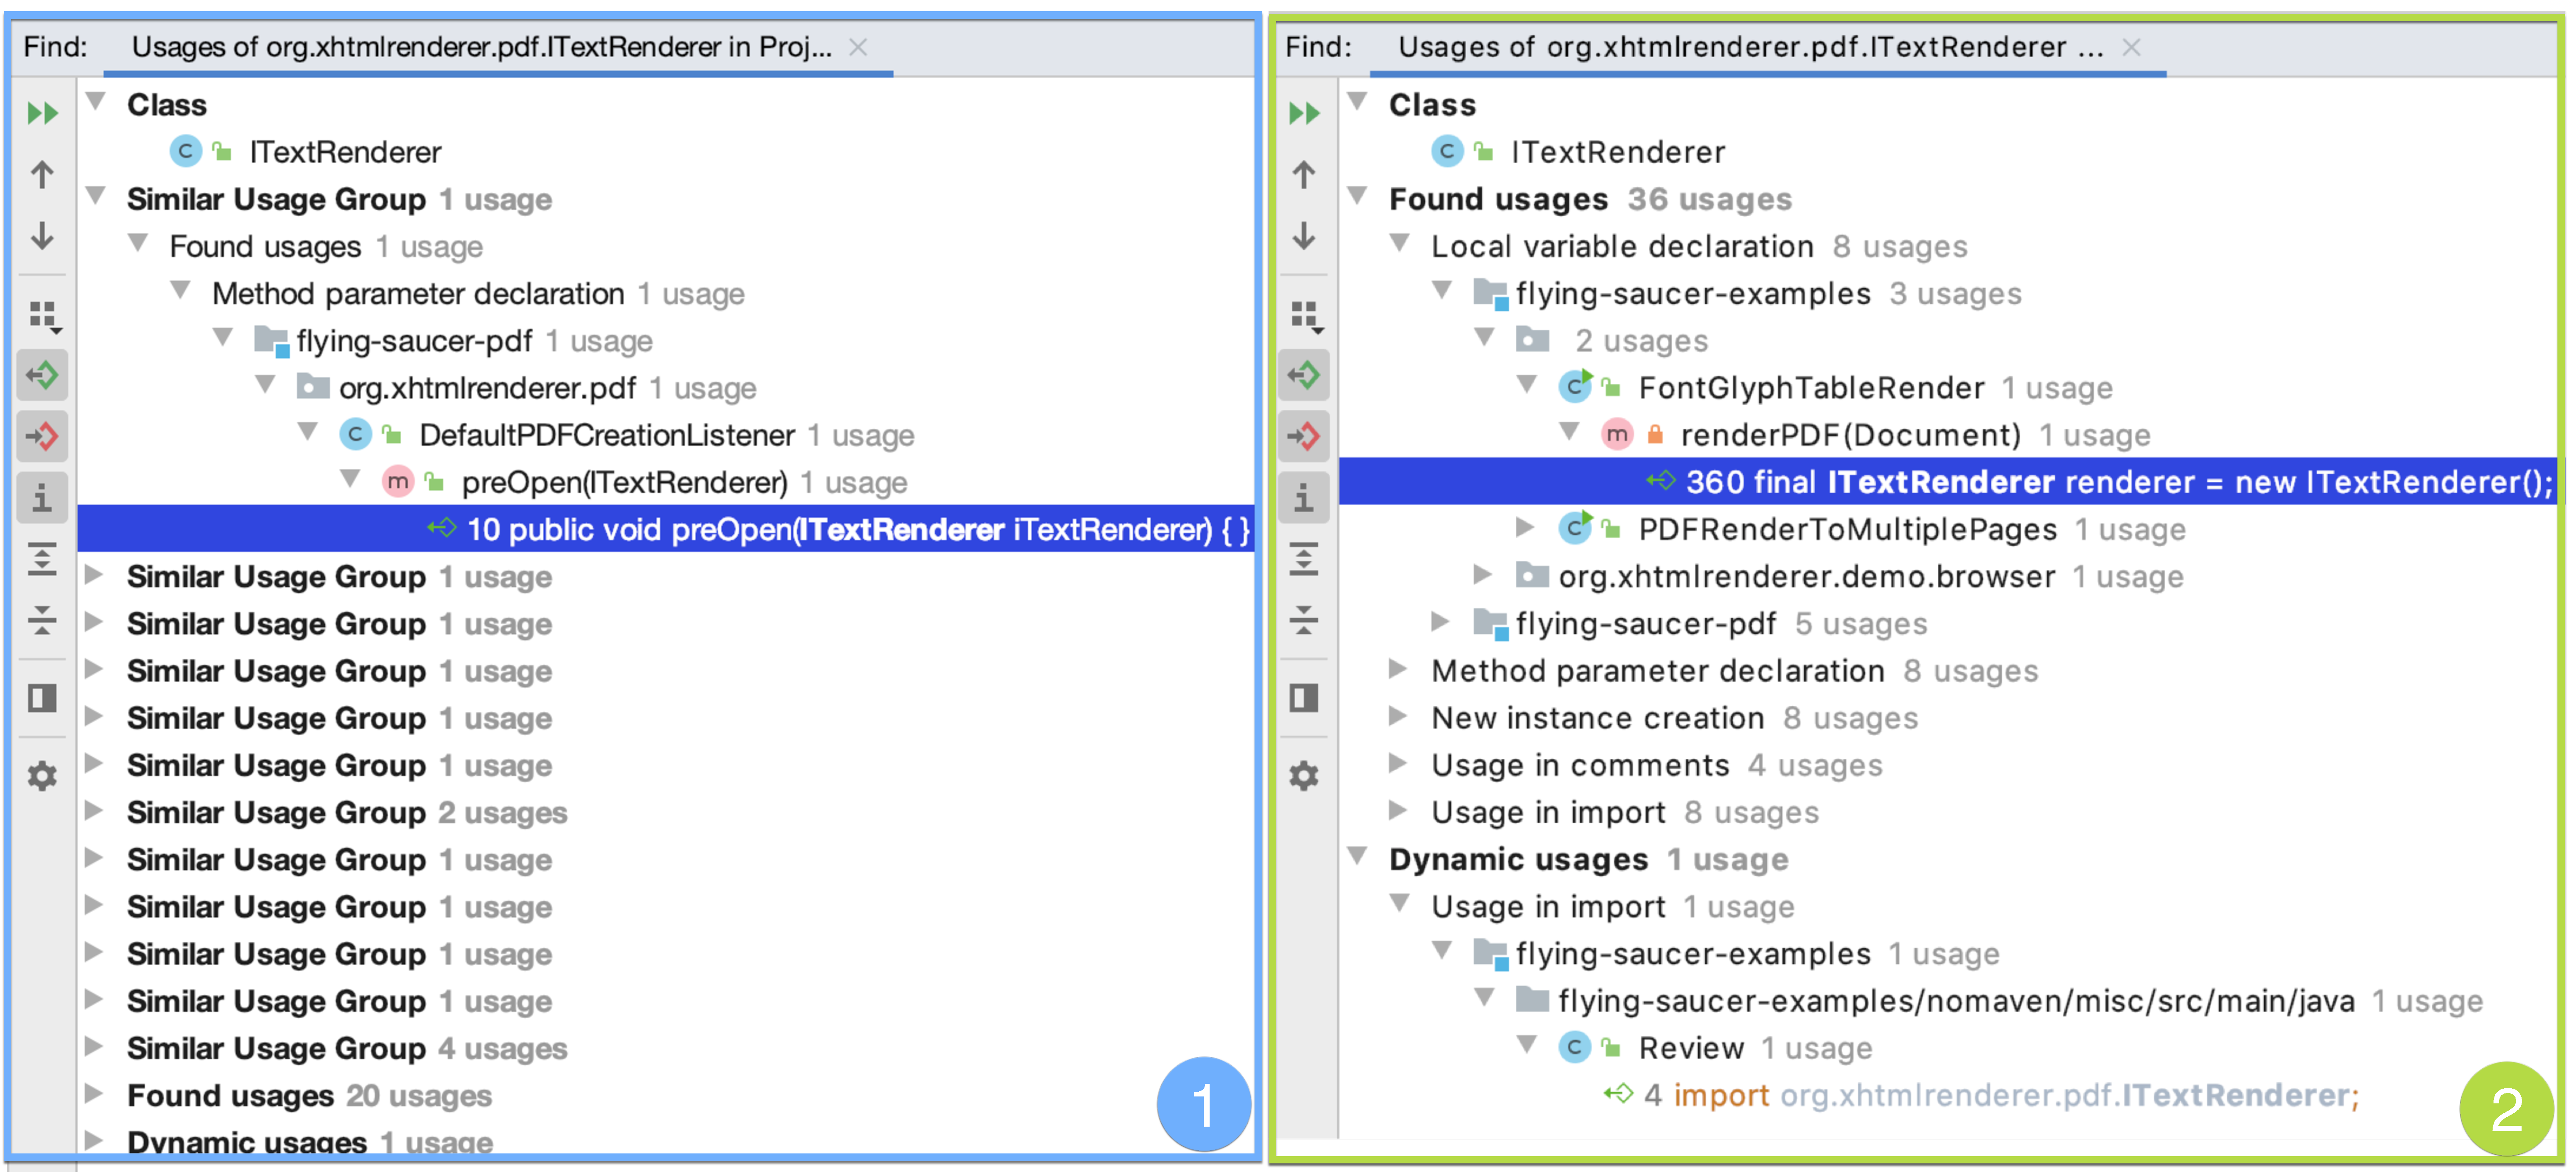
\includegraphics [width=\textwidth,keepaspectratio,clip]{figures/compare}
    \caption{In the blue rectangle number 1 screenshot the interface of Find Unique Usages an the in the number 2 the regular Find Usages are depicted. Both approaches open and highlight the first usages, but the Find Unique Usages group them based on ASTs similarity. It helps developer to donot waste their time for reading duplicate results.  }
\label{fig:compare}
\end{figure*}

\subsection{Results}
To investigate the impact of using Find Unique Usages, we measure the completion time of the task. All participants of both conditions could successfully complete the task. Participants in the experimental group completed that task in a median of 21.5 minutes and 33 minutes in the control group. The 6 participants who worked with Find Unique Usages (M = 23.33, SD = 7.65) compared to the 6 participants in the control group (M = 32.33, SD = 9.35) need significantly lower time for completion tasks. The t-value is 1.82366. The p-value is 0.049094. The result is significant at p \textless 0.05.\par

A qualitative data the behaviors of developers might be useful. We observed the behaviors of developers and labeled them to find a pattern from their activities while they were working on the task. The below behaviors are shared between both the control and experimental group. The reason that they had many common behaviors was the user interface for our tool, and the regular Find Usages tool was similar. \par

Several sequential using of Find Usages tool or Find Unique Usages are misleading. After participants selected a usage, they clicked on that usages and opened the class that contained that usage. In that class, they use another Find Usages on other methods. Sometimes they called Find Usages several times, and they forgot the call graph and got lost. Thus they left the usage and came back to the list of results. After that, they move to another usage. \par

Inline Find Usages might be more useful than seeing results in a separate result window. IntelliJ IDEA has inline Find Usages by pressing control on the keyboard and clicking by mouse on the method that shows a list of usages. In this approach, developers do not go to a separate result window. The result of this approach has a better abstraction. One developer from control group that used this approach she completed the task in 17 minutes. Seventeen minutes was the second minimum of time among the completion time of all participants. Another developer that used this approach was from the experimental group. He completed the task in 13 minutes, which was the lowest among 12 participants. \par

Usages that they accept primitive type like integer are easier to understand than usages they have variables in their input arguments. Results of Find Usages that they have a variable as input parameters, not primitive types, were forcing developers to open the class and read the class to understand the usage. Almost all participants repeated this behavior. They clicked on usage that it had an object as an input argument. Next, they went to the class that the object was an instance of that class. After that, they scrolled over the class's methods and read the code of the class. Sometimes they  (not all participants) called another Find Usage on that class for understanding some methods in that class. It was not clear for experimenters that participants could successfully understand that class or not, but multiple participants loudly said something that I have got lost, which experimenters interpreted that as they failed in the understanding of that class. In the end, participants who were either successful or unsuccessful in understanding the class close that class and come back to the first usage. Since they called another Find Usages, they spent time remembering where they were. Again they called the Find Usage over the first method they were working but left it and went inside a usage. Their behavior was a loop on following activities of going to one usage, clicking on a class, calling anther to find usages, reading code, returning back to the start point. \par

Ua\par

Participants did not skim all results of usages in the beginning. They read result of usages sequentially. They start from the first result in the list then go through the other. The reason that developers start with the first usages is that Find Usages window of IntelliJ IDEA expand and highlight with blue color the first usage. \par


Almost all participants of both conditions had challenges with overloading. In their task they needed to use a method that it was overloaded. The methods had same name, but they had different number of input parameters or type of input parameters or both. When participants were trying to get the usage, this kind of usage was confusing for them.\par

There was a pattern for productive participants, 1) They utilized Find Usages with Find In Path tools for understanding the codebase.  2) Before start reading usages, they expand usages and skimmed the list of usages. After that decided to go through the best usage that might help them. \par

At the end of the study, we interviewed all participants and asked them to tell us about their experiences. One participant told us that several sequential using of Find Usages tool is misleading.
\begin{quote} "I was getting lost when I was using nested [several sequential] Find Usages for understand codebase." - (C6)\end{quote}

 An interesting usability issue that C6 and E3 had with regular Find Usages was the number in the result that shows the line of the statement. They told us they thought this number is the frequency of repeating that statement.\par
 
We received feedback about the grouping of usages in our approach. Find Unique Usages tool used a similar name for all groups in the list of results (see Fig.~\ref{fig:compare}). It was confusing for 2 of participants (E2 and E4). They suggested us to change the naming convention. Since the name of all groups was similar (see Figure.~\ref{fig:compare}) they were curious how we grouped the usages.\par

Also, we asked them to give us any suggestion that might be useful. Participants gave us a couple of suggestions. The interesting one was C6 told us if they have Call Graphs in combination with Find Usages might be useful. He said Call Graph is a useful tool for understanding large codebases, and I am using Call Graph for understanding them. He told us,  the Call Graph helps to get an abstract view over methods.  Also, he said in this way, developers ignore investigation on some methods and spend most of their time focusing on the basic methods. While C6 was working on his tasks, he called several sequential Find Usages for understanding the code. Then he said he has got lost. At the end of the study, he said if he had had a Call Graph, probably he would not have got lost in usages.     


% *************************Limitation********************************************************************
\section{Limitation And Threats To Validity}
Our study had several limitations and potential threats to the internal and external validity of the results. \par  

In selecting a task, we sought to identify a task that is representative of a typical large codebase that contains many usages for methods. Smaller or Larger codebase may involve more complex usages where individual behaviors are more challenging to identify. \par 

The second threat is Find Unique Usages approach is dependent on IDE and language. It is not clear if we use it on other IDEs or other languages, the result might be different.\par 

% *************************Discussion********************************************************************
\section{Discussion}
Our exploratory study showed there exist challenges in Find Usages tool of IntelliJ IDEA. We designed an approach and implement a tool on top of Find Usages tool of IntelliJ IDEA to fix the issues. Our approach utilize AST diffs of usages for grouping similar usages in one group. The result of controlled experiment showed our approach could decrease 35\% of time completion of implementation a simple logic in a large codebase.

The approach that we used for grouping the usage was a naive approach to clustering that we took due to time constraints preventing us from better understanding the IntelliJ SDK. In the future, we hope to re-implement the usage grouping with merging as part of an agglomerate clustering approach. Also, We can work on scalability and response time of the tool \par


A couple of participants complaint about the naming convention of groups. The names of the groups were similar. In future, we must change it to more readable names.\par

IntelliJ IDEA by default expand and highlight the first usages in the list of result. It is not clear what would be behaviors of developers if IDE does not highlight the first usage. A future investigation might be, if Find Usages tool expands all usage by default and do not highlight the first uasge what would be the bevaiors of developers.\par

IntelliJ IDEA had inline Find Usages tool, which looks great. We did not think about it. Nevertheless, we guess developers who use the inline Find Usages might be more productive. In the future, we might compare them. \par

In future work, this should either be picked based on trying out different thresholds on different projects or probably better, allowing it to be configured by a menu option as part of the IDE plugin. Choosing the similarity threshold here for describing similar code, is also familiar to choosing a K when doing K-means, which depends highly on the data-set that K-means is applied to. Picking a reasonable default threshold would be future work, but for now, the best approach would probably be to set it as an option via a menu.

% *************************Conclusion********************************************************************
\section{Conclusion}
Developers have difficulties in understanding the context of how various internal classes, objects, or methods are used in the codebase. We sought to better understand these challenges by conducting a think-aloud user study with 6 participants. The results of the think-aloud experiment highlighted that developers spend considerable time learning to use internal code artifacts. The result also showed developers use the Find Usages/References tool of IDEs to understand code by example. The results of Find Usages can be long tail of results that developers find difficulty mentally parsing. We also found that find usage/reference results' would contain duplicate examples in disparate locations in the UI, adding to the difficulty of parsing. Based on the think-aloud study. We designed and implemented Find Unique Usages, which groups usages  manipulated result of Find Usages and grouped them based on their similarity. After that, we conducted a controlled experiment with 12 more participants to evaluate our approach. Results showed that this aggregation of Unique examples save 35\% times of developers..


% \section*{Acknowledgment}
% % [TODO]: mention Dr. Jon Bell. He helped us in first ideation part of the paper.
% acknowledgments in the unnumbered footnote on the first page.

\bibliographystyle{IEEEtran}
\bibliography{FUU}



\end{document}
